
%##########################  Inicio encabezado  ##########################%

\documentclass{article}[12pt, a4paper]
\usepackage{amsfonts,amssymb,amsthm,amsmath}%paquetes para simbolos
\usepackage[latin1]{inputenc}%espa\~nol
\usepackage[spanish]{babel}%espa\~nol
\usepackage{graphicx}
\usepackage{tikz}
\usetikzlibrary{positioning}
\setlength{\textwidth}{430pt}
\addtolength{\hoffset}{-20pt}

\title{Trabajo Pr\'actico N� 3}
\author{Bugnon, Leandro \and Pineda, Leandro \and Rodriguez, Tadeo}
\date{}
\newcommand{\norma}[1]{\left\|#1\right\|^2}
\newcommand{\ejr}[1]{\section*{Ejercicio #1}}

\begin{document}
%\maketitle
%##########################  Inicio car�tula  ##########################%



%88888888888888888888888888  Fin Car�tula  88888888888888888888888888%
\maketitle
El desarrollo de las redes neuronales profundas, mediante la incorporaci\'on
de capas convolutivas, ha significado un avance sustancial en el \'area de
aprendizaje supervisado de imagenes. Por ejemplo, la red neuronal profunda
esquematizada en la Figura~\ref{redorig} logra una exactitud $99.25\%$ sobre
un conjunto de datos de 10 clases que representan digitos manuscritos (MNIST).



\begin{figure}[h]
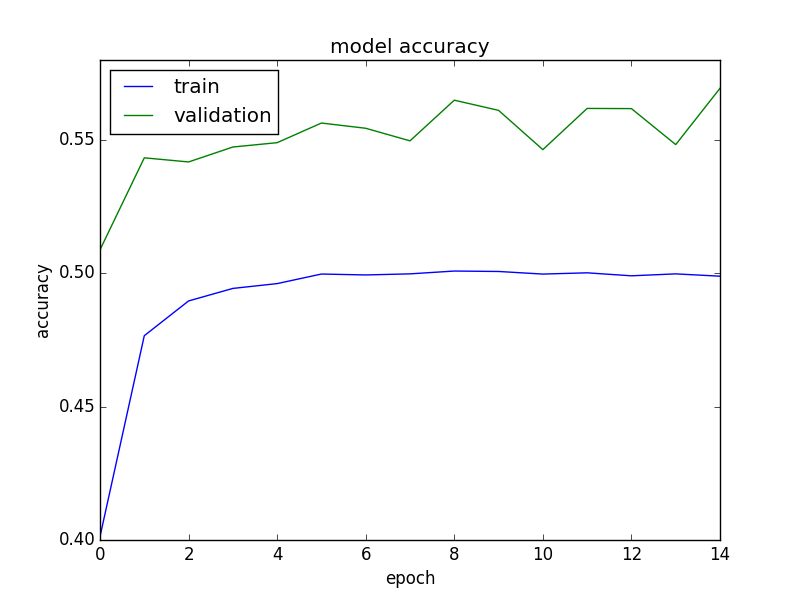
\includegraphics[width=400pt,height=150pt]{ej1acc}
\label{redorig}
\caption{Red neuronal profunda MNIST. $99.25\%$ de exactitud.}
\end{figure}
Considerando el ejemplo de los digitos,
se desea hacer lo mismo con caracteres de un texto manuscrito. Dicho conjunto de datos fue extra\'ido
de imagenes de textos completos, que fueron posteriormente segmentados. Dicha segmentaci\'on es aproximada,
pues no es posible dividir cada uno de los caracteres en forma apropiada. Por otra parte, los textos
fueron escritos por diferentes individuos, lo que implica un dataset de gran tama\~no y diversidad.
A su vez, se optado por separar los autores, un conjunto ser\'a destinado al entrenamiento/validaci\'on y
otro exclusivamente al testeo. De esta manera el clasificador tendr\'a el desafio de clasificador
ejemplos que en ning\'un momento utilizo durante se entrenamiento, ni si similares que hubieren
provenido del mismo escritor.

A tal fin, se parte del modelo propuesto para MNIST con la modificaciones necesarias para ser utilizada
en este conjunto de datos. En particular, se modifica la \'ultima capa de neuronas cuya arquitectura
esta definida por la cantidad de clases. En este caso existen 91 clases en lugar de las 10 del ejemplo
anterior. Los resultados de este sencillo modelo pueden ser apreciados en la Figura~\ref{ej1}. Lo obtenido
difiere significamente de lo logrado en MNIST \--- por la cantidad de clases y el desbalance de las mismas,
entre otros motivos\--- y representa un punto de partida sobre el cual
realizar modificaciones para as\'i lograr una mejor performance. Por lo tanto, la estrategia consistir\'a
en modificar individualmente cada uno de los para\'ametros del modelo, indagando el efecto de cada
uno en la performance general. Finalmente, a partir del conocimiento inferido, se buscara exhaustivamente
una arquitectura apropiada para el problema de inter\'es.

En primer lugar, la estrategia que se adopta consiste en realizar  un preprocesamiento de los datos. 
En particular se opta por realizar un escalado de los datos, asi como una transformaci\'on en escala
de grises. A tal fin se utilizan las herramientas de preprosamiento de Keras. Esta rutina logra una mejora
en la performance, de alrededor de 5 puntos con respecto al modelo original, como se puede apreciar
al comparar la Figura~\ref{ej2} con la anterior. Asimismo, este procedimiento es normal, por lo que se
decide incluirla en el resto de las realizaciones del m\'etodo.
\begin{figure}[h!]
	\begin{minipage}[h]{0.49\textwidth}
		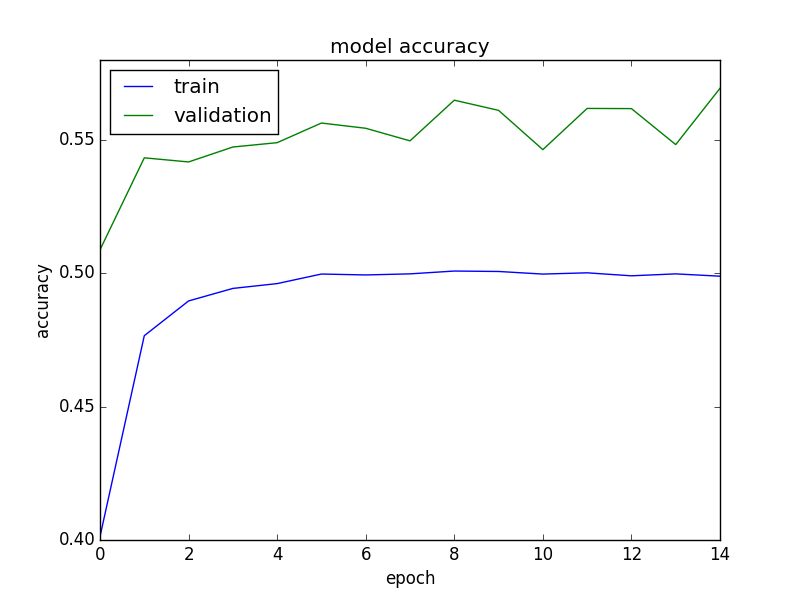
\includegraphics[width=\textwidth]{ej1acc}
	\end{minipage}
	\begin{minipage}[h]{0.49\textwidth}
		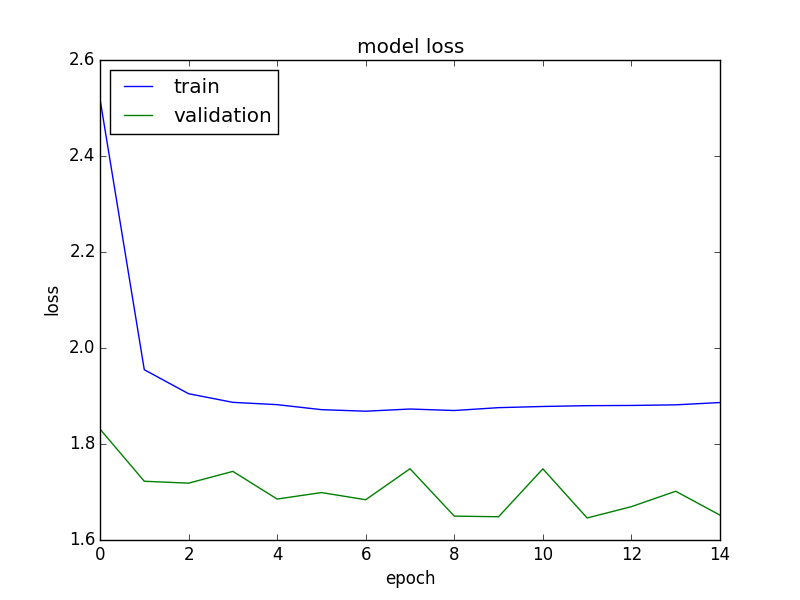
\includegraphics[width=\textwidth]{ej1loss}
	\end{minipage}
	\caption{Exactitud y perdida. Red basada en MNIST.}
	\label{ej1}
\end{figure}

\begin{figure}[h!]
	\begin{minipage}[h]{0.49\textwidth}
		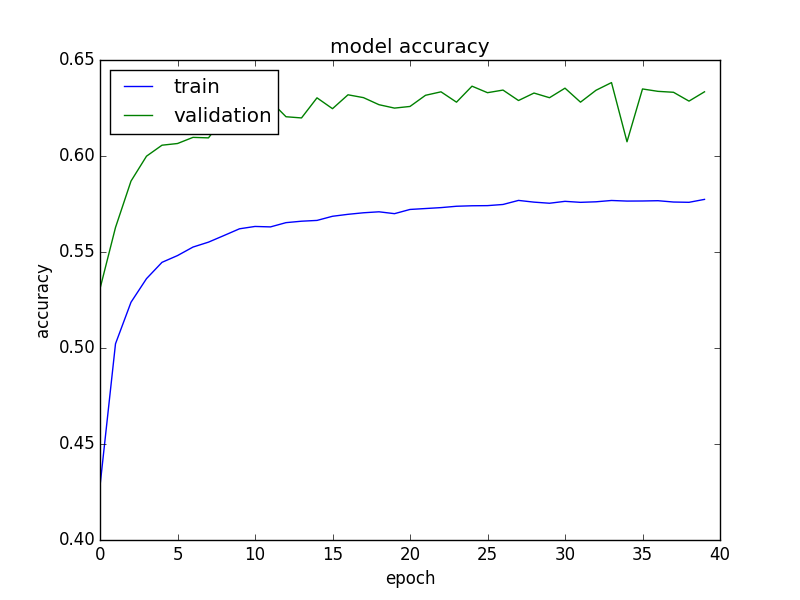
\includegraphics[width=\textwidth]{ej2acc}
	\end{minipage}
	\begin{minipage}[h]{0.49\textwidth}
		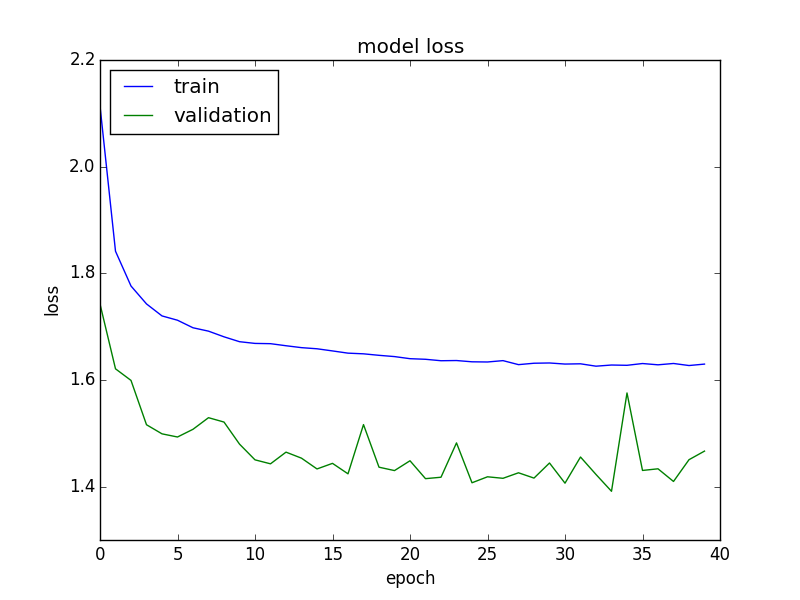
\includegraphics[width=\textwidth]{ej2loss}
	\end{minipage}
	\caption{Exactitud y perdida. Aplicando preprocesamiento.}
	\label{ej2}
\end{figure}
\vfil
\newpage
Por otra parte, resulta de inter\'es analizar el comportamiento de la red,
con un porcentaje de los datos de entrenamiento. Esta observaci\'on nos permite
prevenir defectos en el modelo como es el caso del overfitting o similares. En
este caso se utiliz\'o un 25\% de los datos disponibles para entrenamiento. Como
se ve en la Figura~\ref{ej3a}, esta disminuci\'on no representa una mejor\'ia del
desempe\~no respecto al caso anterior. Esta situaci\'on puede entenderse debido a la
presencia del Dropout, el cual previene de los inconvenientes mencionados.

\begin{figure}[h!]
	\begin{minipage}[h]{0.49\textwidth}
		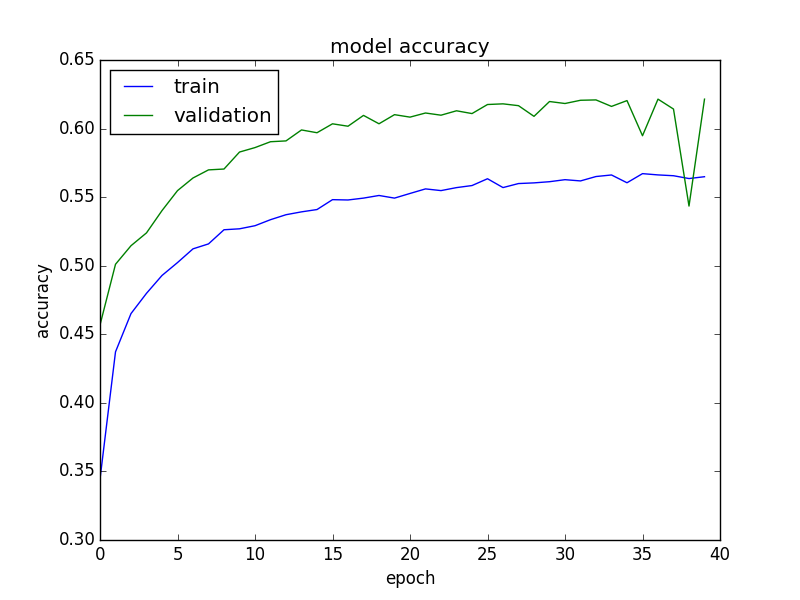
\includegraphics[width=\textwidth]{ej3acc}
	\end{minipage}
	\begin{minipage}[h]{0.49\textwidth}
		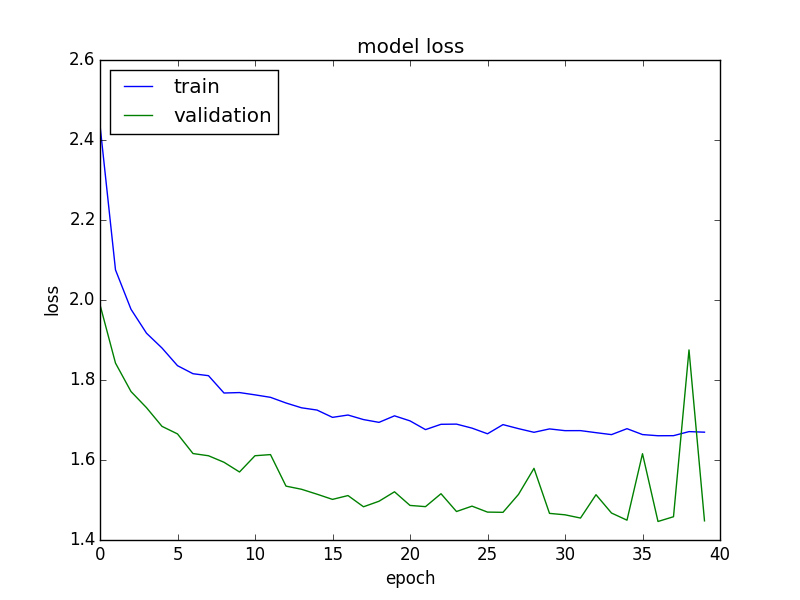
\includegraphics[width=\textwidth]{ej3loss}
	\end{minipage}
	\caption{Exactitud y perdida. Red original utilizando un 25\% de los datos de entrenamiento.}
	\label{ej3a}
\end{figure}

Uno de los par\'ametros mas influyentes de una red neuronal profunda es la arquitectura
que toman sus capas convolutivas. La cantidad de filtros y el tama�o de los mismos as\'i
como el n\'umero de capas convolutivas juegan papel preponderante en el dise�o y funcionamiento
de este tipo de red. En particular se medir\'a el desempe�o de estas, en el caso extremo de una
sola capa convolucional y en un caso con 5 capas convolutivas. En ambos, las capas poseen 32 filtros
de $3\times3$ pixeles. Estan colocados de manera secuencial, y seguidos por una capa de Maxpooling,
en forma similar al modelo original.

El resultado de ambas se puede apreciar en las Figuras~\ref{ej3b1}~y~\ref{ej3b2}. All\'i se observa que
la sustracci\'on de una capa respecto al modelo original implica, una perdida de alrededor de 5 puntos
porcentuales de exactitud. En cambio, la adici\'on de capas permite aumentar en 5 puntos, respecto al modelo
con preprocesamiento. 

\begin{figure}[h!]
	\begin{minipage}[h]{0.49\textwidth}
		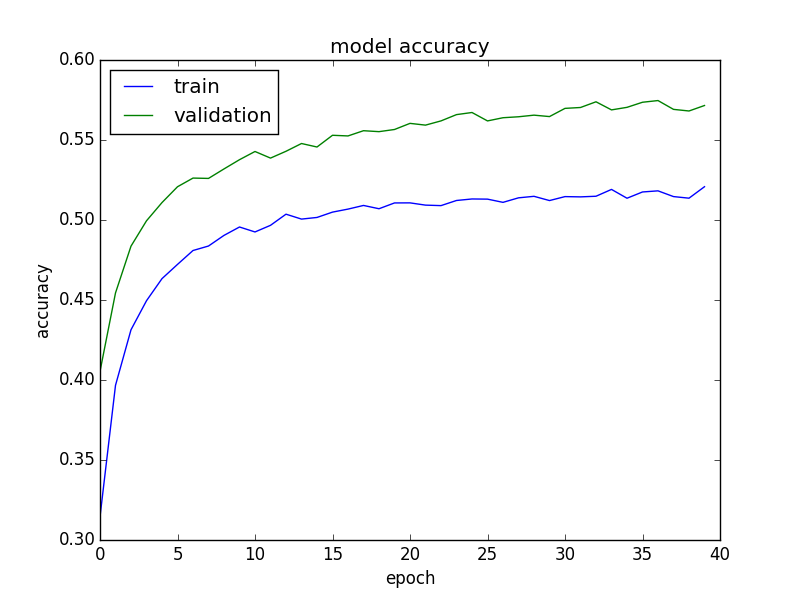
\includegraphics[width=\textwidth]{ej3b1acc}
	\end{minipage}
	\begin{minipage}[h]{0.49\textwidth}
		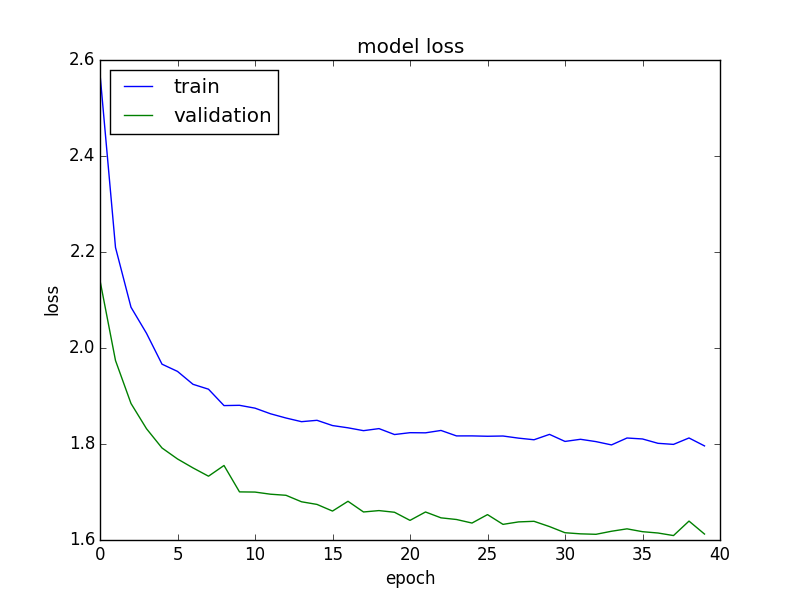
\includegraphics[width=\textwidth]{ej3b1loss}
	\end{minipage}
	\caption{Exactitud y perdida. Red con una sola capa convolutiva}
	\label{ej3b1}
\end{figure}
	

\begin{figure}[h!]
	\begin{minipage}[h]{0.49\textwidth}
		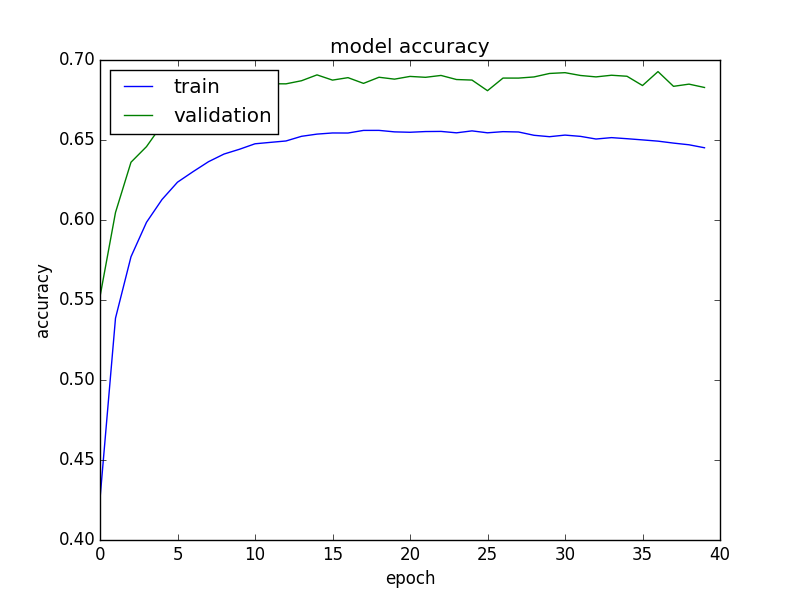
\includegraphics[width=\textwidth]{ej3b5acc}
	\end{minipage}
	\begin{minipage}[h]{0.49\textwidth}
		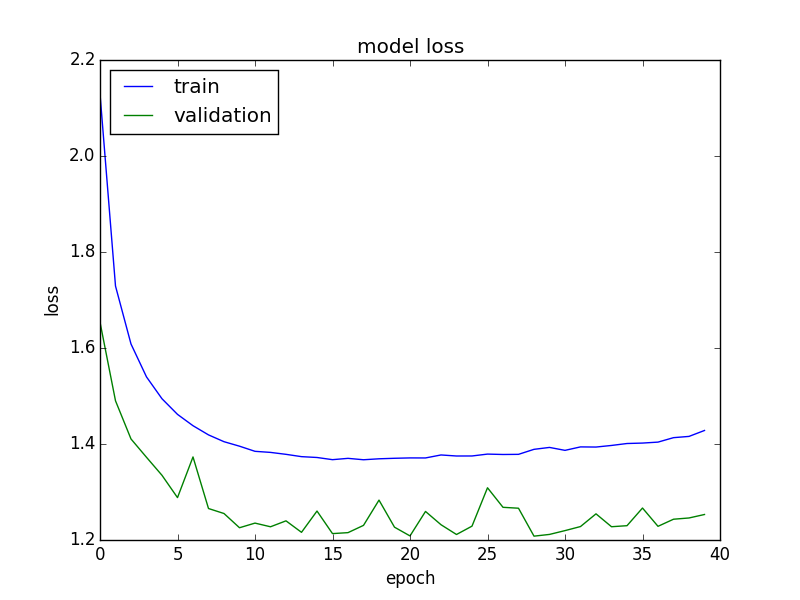
\includegraphics[width=\textwidth]{ej3b5loss}
	\end{minipage}
	\caption{Exactitud y perdida. Red con 5 capas convolutivas.}
	\label{ej3b2}
\end{figure}
	
El otro par\'ametro mas significativo de este tipo de red, se trata del clasificador mismo, las
capas completamente conectadas al final de la red. Estas representan casi la totalidad de par\'ametros
que deben ser ajustados en el modelo, influyendo no solo en el desempe�o sino tambie\'en en el tiempo
de entrenamiento. El modelo actual, consta de una sola capa oculta con 100 neuronas. La estrategia que se
adopta, y cuyos resultados se muestran en Figura~\ref{ej3c1}, es reducir la cantidad neuronas a 32. Por otro lado
se desea conocer el efecto de tener mayor cantidad de capas ocultas. En la Figura~\ref{ej3c2} se ve la performance
de una red con 3 capas ocultas de 256, 128 y 64 neuronas cada una. Claramente ambas opciones representan
un decaimiento en la calidad de la clasificaci\'on, siendo la mas significativa para el caso de la disminuci\'on
de neuronas.

\begin{figure}[h!]
	\begin{minipage}[h]{0.49\textwidth}
		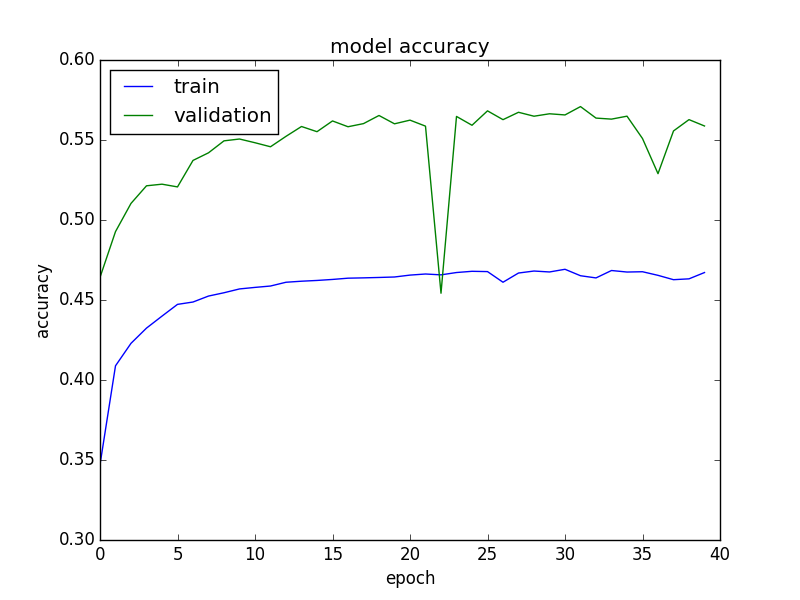
\includegraphics[width=\textwidth]{ej3clessacc}
	\end{minipage}
	\begin{minipage}[h]{0.49\textwidth}
		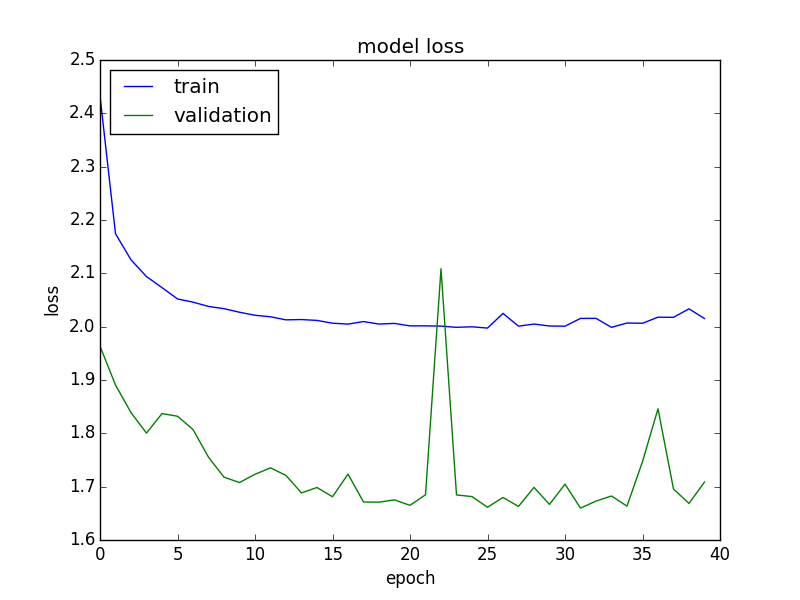
\includegraphics[width=\textwidth]{ej3clessloss}
	\end{minipage}
	\caption{Exactitud y perdida. Red con una capa totalmente conectada(32).}
	\label{ej3c1}
\end{figure}
	

\begin{figure}[h!]
	\begin{minipage}[h]{0.49\textwidth}
		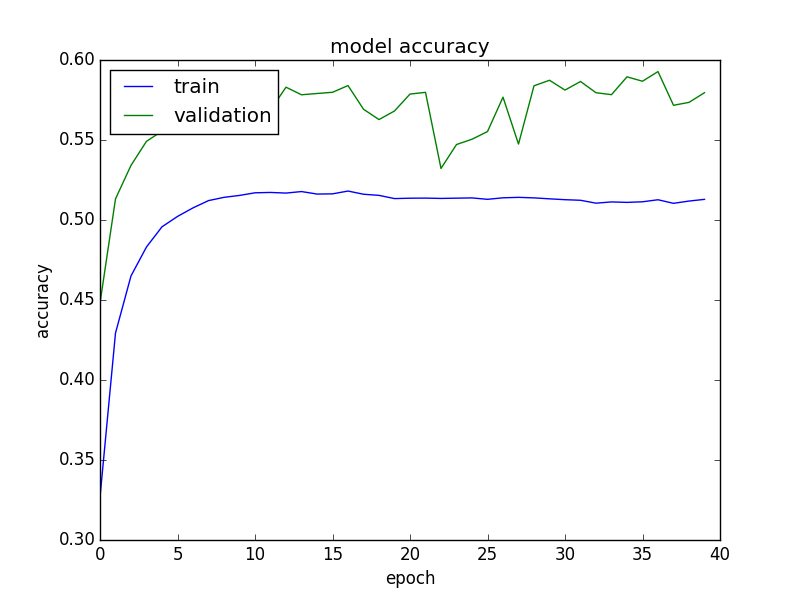
\includegraphics[width=\textwidth]{ej3cmoreacc}
	\end{minipage}
	\begin{minipage}[h]{0.49\textwidth}
		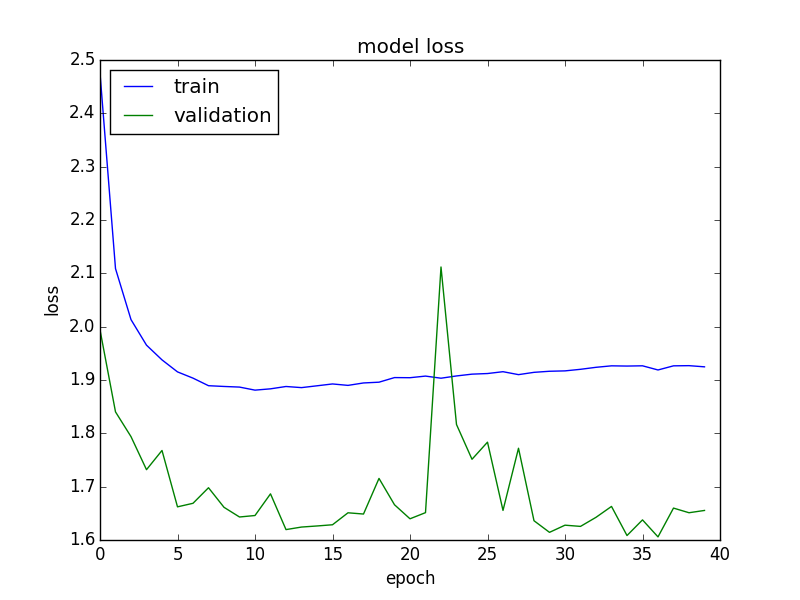
\includegraphics[width=\textwidth]{ej3cmoreloss}
	\end{minipage}
	\caption{Exactitud y perdida. Red con 3 capas totalmente conectadas(256,128,64).}
	\label{ej3c2}
\end{figure}

\newpage
Otra elecci\'on que puede influir en el funcionamiento del modelo es la
funci\'on de activaci\'on escogida. En la red base, todas las activaciones
son del tipo \textit{ReLU}. Otra posibilidad es utilizar funciones sigmoideas
es decir la funci\'on:
\[\mathrm{sigmoid}(x)=\frac{1+\tanh{x}}{2}=\frac{e^x}{e^x+e^{-x}}.\]

El efecto de esta sustituci\'on se puede apreciar en la Figura~\ref{ej3d}
donde se observa un fuerte decaimiento en la calidad del clasificador,
desempe�andose a\'un peor que el modelo sin preprocesamiento. De esta
manera se puede afirmar que la RELU ser\'a una mejor opci\'on en el
momento de construir un modelo con el mayor desempe�o posible para esta
dataset.

\begin{figure}[h!]
	\begin{minipage}[h]{0.49\textwidth}
		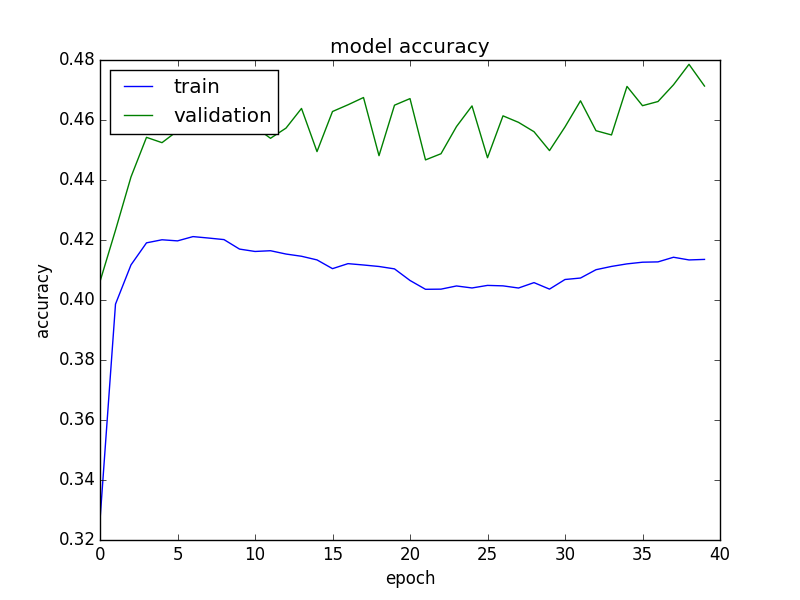
\includegraphics[width=\textwidth]{ej3dacc}
	\end{minipage}
	\begin{minipage}[h]{0.49\textwidth}
		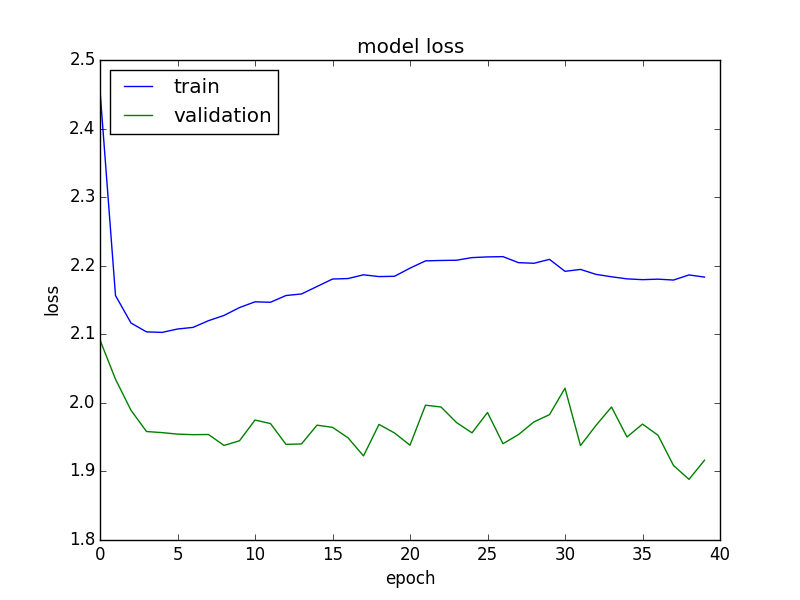
\includegraphics[width=\textwidth]{ej3dloss}
	\end{minipage}
	\caption{Exactitud y perdida. Red con funciones sigmoideas en la activaci\'on.}
	\label{ej3d}
\end{figure}

\newpage
Finalmente, otra caracter�stica que se desea analizar es el efecto del Dropout.
Este tiende a disminuir los errores por overfitting, sin embargo, resulta de inter�s
conocer si el nivel es apropiado o, incluso, si su efecto es en realidad negativo
en la cosntrucci\'on del modelo.

Las curvas en las Figuras~\ref{ej3e}~y~\ref{ej3f} dejan en claro que aumentar
el Dropout empeora el comportamiento del modelo, mientras que eliminarlo
significa un aumento significativo respecto al modelo base pero, posiblemente,
sensible al overfitting

\begin{figure}[b]
	\begin{minipage}[h]{0.49\textwidth}
		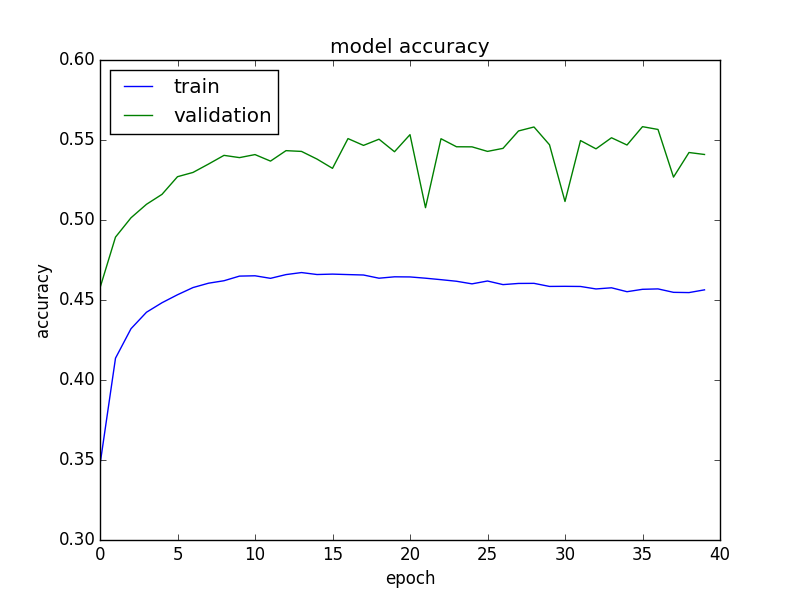
\includegraphics[width=\textwidth]{ej3eacc}
	\end{minipage}
	\begin{minipage}[h]{0.49\textwidth}
		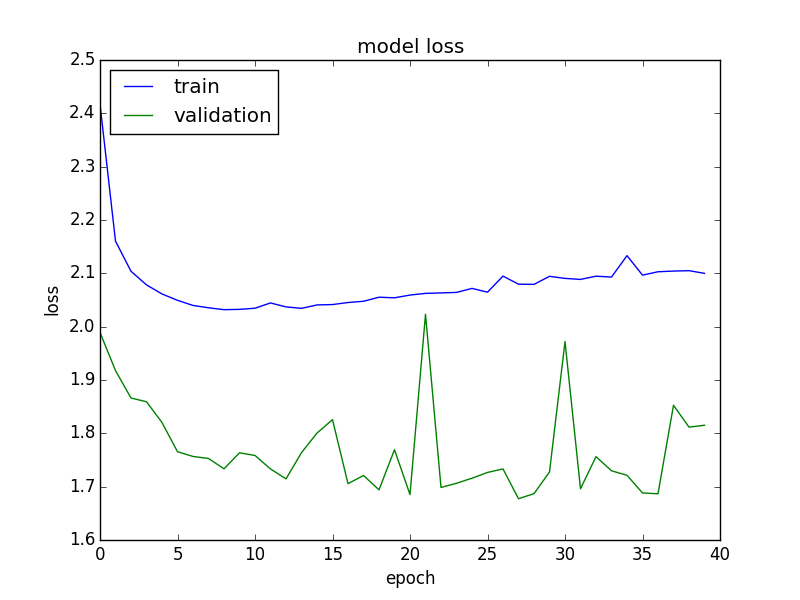
\includegraphics[width=\textwidth]{ej3eloss}
	\end{minipage}
	\caption{Exactitud y perdida. Red con nivel de Dropout aumentado.}
	\label{ej3e}
\end{figure}

\begin{figure}[b]
	\begin{minipage}[h]{0.49\textwidth}
		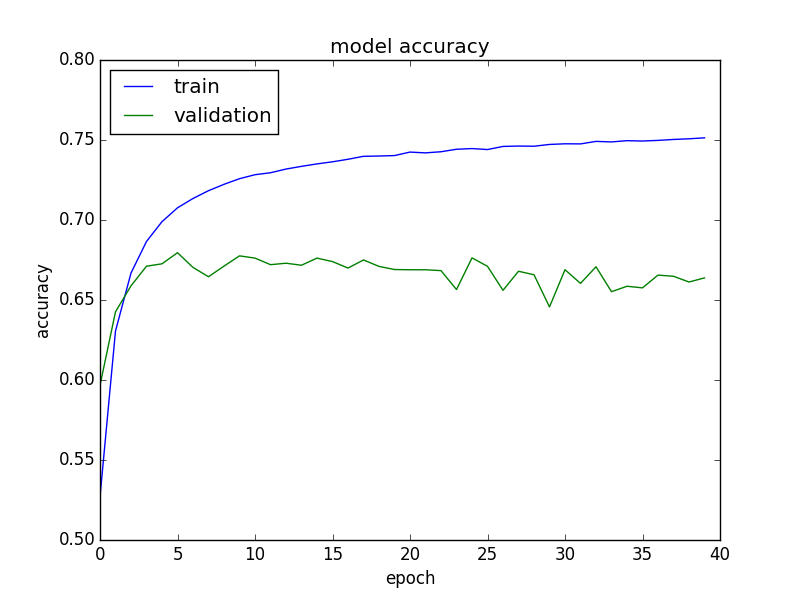
\includegraphics[width=\textwidth]{ej3facc}
	\end{minipage}
	\begin{minipage}[h]{0.49\textwidth}
		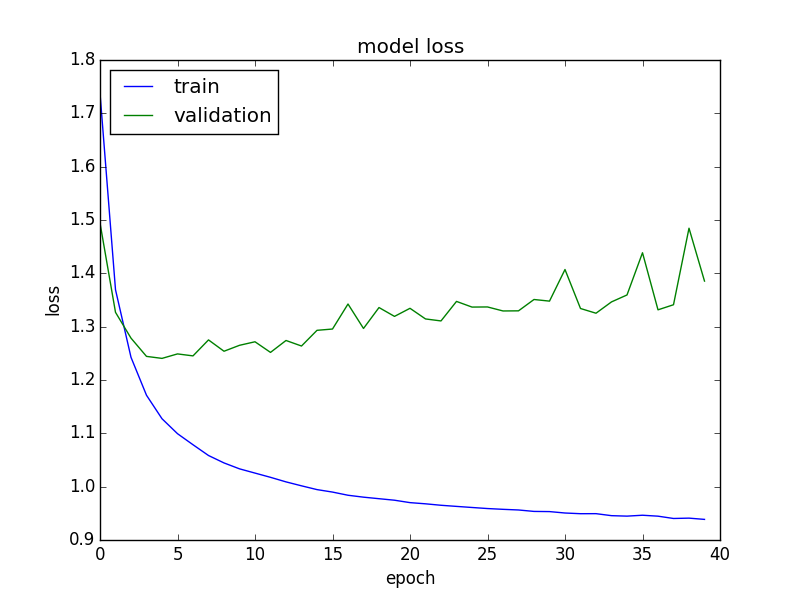
\includegraphics[width=\textwidth]{ej3floss}
	\end{minipage}
	\caption{Exactitud y perdida. Red sin efecto de Dropout.}
	\label{ej3f}
\end{figure}

\end{document}